\chapter{Implementazione} %\label{1cap:spinta_laterale}
% [titolo ridotto se non ci dovesse stare] {titolo completo}
%

\begin{citazione}
In questo capitolo verrà illustrato come è stato possibile implementare la soluzione proposta e verranno illustrati anche i risultati che sono stati ottenuti
\end{citazione}

\section{Scelta del protocollo}
Al fine di procedere con il lavoro di messa in sicurezza è stato necessario scegliere uno dei protocolli \emph{Automotive} disponibili in letteratura. La prima scelta è stata \emph{FlexRay} in quanto è il protocollo più promettente e con hardware più prestante ma, sfortunatamente, dopo un'attenta ricerca in rete non è stata trovata nessuna implementazione software del protocollo. Erano disponibili solo all'acquisto delle \emph{board di testing} (con costi anche abbastanza sostanziosi) che permettevano di simulare il protocollo tramite strumentazione adeguata. Non avendo avuto fortuna con \emph{FlexRay}, la seconda scelta è ricaduta su \emph{LIN}. Purtroppo anche qui non è stato possibili trovare implementazioni \textbf{funzionanti} e \textbf{complete} del protocollo, ma solo tentativi abbandonati di implementarlo. Per queste ragioni, infine, si è scelto il protocollo \textbf{\emph{CAN}} che è supportato in maniera nativa dal kernel \textbf{Linux} tramite dei moduli appositi (oltre ad avere anche diverse implementazioni software complete e funzionanti), permettendo persino la creazione di uno o più nodi virtuali.

\section{Soluzione proposta}
Per cercare di risolvere il problema della mancanza di sicurezza all'interno del protocollo \emph{CAN}, quello che si è voluto proporre è l'\textbf{aggiunta di uno strato di cifratura} che proteggesse lo scambio di messaggi sulla rete. In particolare, si è deciso di impiegare \textbf{cifrari post-quantum} sia per garantire la massima sicurezza contro la maggior parte degli attacchi noti in letteratura sia per stabilire quale possa essere l'impatto sulle prestazioni. In seguito a questa decisione, quindi, si è deciso di impiegare per la soluzione il cifrario \textbf{AES-256} per gestire la parte di cifratura dei messaggi e \textbf{CRYSTALS-kyber-512} per far accordare i nodi della rete su una stessa chiave di sessione da utilizzare per cifrare e decifrare i messaggi.

Sostanzialmente è stato implementato un \textbf{cifrario ibrido}, ovvero un cifrario che ha una componente asimmetrica per far accordare i nodi su una stessa chiave di sessione e che ha una componente simmetrica con la quale viene utilizzata la chiave di sessione come chiave di cifratura per i messaggi che devono essere scambiati. La ragione di un cifrario del genere riguarda le \textbf{prestazioni}, poichè i cifrari asimmetrici sono estremamente più lenti dei cifrari simmetrici e, per questa ragione, non è conveniente gestire lo scambio di messaggi utilizzando solo un cifrario asimmetrico.

\section{Implementazione}
Al fine di valutare le prestazioni e la fattibilità della soluzione proprosta, è stato realizzato un applicativo molto elementare che realizza le operazioni crittografiche e utilizza \emph{CAN} per inviare dati e messaggi. Il codice contenente l'applicativo, le dipendenze e un tester può essere consultato nella repository al seguente indirizzo: \url{https://github.com/lorycris99/tesi-magistrale}.

Per l'implementazione è stato scelto di utilizzare il linguaggio \textbf{C} sia perchè le implementazioni di \emph{CAN} e delle primitive crittografiche utilizzate sono disponibili principalmente in questo linguaggio e sia per via della sua efficienza, in modo da avere una stima delle prestazioni più "realistica" possibile (solitamente anche gli applicativi reali sono scritti in \textbf{C}). Inoltre, per effettuare la compilazione dell'applicativo è necessario tener conto di alcuni accorgimenti:
\begin{itemize}
    \item Il sistema operativo su cui è stato realizzato e testato è \textbf{Ubuntu}, per cui su sistemi diversi come \textbf{Windows} non sarà possibile utilizzarlo;
    \item Dal momento che l'applicativo necessita di dipendenze che non sono presenti nei percorsi di default del \textbf{Linker}, è necessario istruirlo su dove trovare le varie librerie. Osservando il \autoref{lst:linker-info} si può vedere il comando da inviare per compilare correttamente, dove con \texttt{-L/path/to/lib} si indica la cartella dove si trovano le librerie che verranno indicate e con \texttt{-l:lib.so} si indica il nome della libreria da includere;
    \item Oltre ad istruire il \emph{Linker}, è necessario istruire anche il \textbf{Loader} poichè anche se la compilazione va a buon fine, il \emph{Loader} non troverà le librerie specificate al \emph{Linker}. Il comando da eseguire è mostrato nel \autoref{lst:loader-info} e il \textbf{path} da specificare (ovviamente) deve essere lo stesso di quello specificato al \textbf{Linker}.
\end{itemize}

\begin{lstlisting}[keywords={gcc}, caption=Istruzioni per il Linker, label=lst:linker-info]
    gcc test.c ../kyber/ref/randombytes.c -L/path/to/lib -l:libpqcrystals_kyber512_ref.so -l:libpqcrystals_aes256ctr_ref.so -l:libpqcrystals_fips202_ref.so
\end{lstlisting}

\begin{lstlisting}[keywords={export}, caption=Istruzioni per il Loader, label=lst:loader-info]
    export LD_LIBRARY_PATH=/path/to/lib
\end{lstlisting}

\begin{figure}[h]
    \centering
    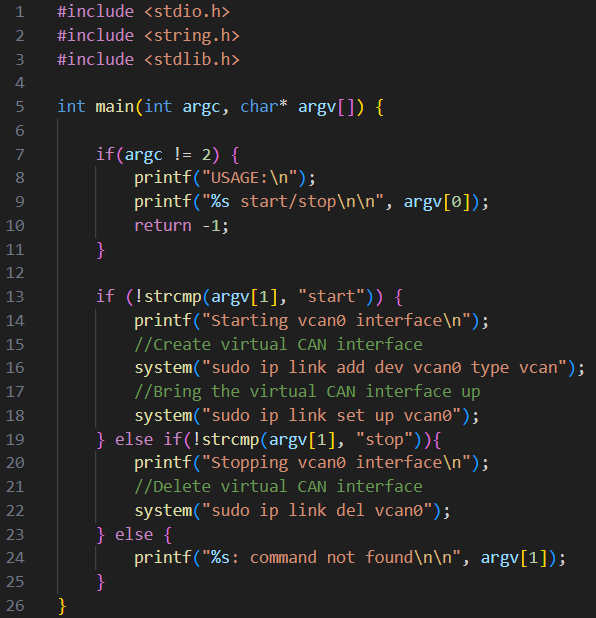
\includegraphics[width=0.6\textwidth]{capitoli/figure-implementazione/can.c.png}
    \caption{Codice sorgente del file \texttt{can.c}}
    \label{fig:can-c-code}
\end{figure}

Una volta istruiti \textbf{Linker} e \textbf{Loader} su dove trovare le librerie, quello che bisogna fare è creare un nodo \emph{CAN} con cui poter comunicare. Per essere in grado di farlo, bisogna innanzitutto abilitare il \textbf{modulo del kernel} interessato lanciando il comando \texttt{sudo modprobe vcan}, successivamente basta compilare ed eseguire il file \texttt{can.c} per avviare il nodo \emph{CAN} virtuale. Il codice del file è illustrato nella \autoref{fig:can-c-code}.


\subsection{Protocollo realizzato}
Poichè quello che si sta cercando di implementare non è presente \textbf{nativamente} in \emph{CAN}, c'è bisogno di una strategia per fare in modo da inserire all'interno del protocollo un metodo per lo scambio di chiavi e per richiedere eventualmente una nuova chiave. Essendo che \emph{CAN} lavora principalmente con gli \textbf{ID} dei messaggi, la strategia più conveniente è stata quella di utilizzare degli \textbf{ID inutilizzati dal protocollo} e assegnarli a dei messaggi \emph{personalizzati} che svolgano le operazioni aggiuntive che si vogliono implementare. Sfortunatamente, non esistono degli ID inutilizzati \textbf{universalmente} in quanto ogni casa automobilistica gestisce gli \textbf{ID} a proprio piacimento per cui bisognerebbe adattare gli \textbf{ID} caso per caso.\\
Ai fini delle simulazioni realizzate, si sono presi degli \textbf{ID bassi} (solitamente sono i meno utilizzati) e si è immaginato che non corrispondano a messaggi già assegnati. Gli \textbf{ID} utilizzati sono stati i seguenti:
\begin{itemize}
    \item $111$: messaggio che indica la presenza di una parte della \textbf{chiave pubblica} nel payload;
    \item $112$: messaggio per richiedere ad un nodo di reinviare la \textbf{chiave pubblica};
    \item $122$: messaggio che indica la presenza di una parte della \textbf{capsula} nel payload;
    \item $123$: messaggio per richiedere ad un nodo di reinviare la \textbf{capsula};
    \item $A$: messaggio che serve ad innescare la generazione di traffico casuale, utilizzato per valutare la correttezza dell'applicativo e delle operazioni di crittografia;
    \item $B$: messaggio generato casualmente e cifrato tramite \textbf{AES-256}, in risposta all'\textbf{ID} $A$;
    \item $0$: messaggio che fa terminare l'applicativo;
\end{itemize}

A questo punto, il prossimo passo è stato ideare un "protocollo" che permetta di scambiare correttamente le informazioni necessarie per concordare una chiave ma sorge anche un problema da risolvere: la lunghezza della \textbf{chiave pubblica} e della \textbf{capsula}. Un messaggio \emph{CAN} è in grado di inviare fino a 8 Byte di dati mentre una chiave pubblica di \textbf{kyber-512} è lunga 800 byte e una \emph{capsula} è lunga 768 byte, per cui la soluzione più semplice è sembrata quella di dividere entrambi in gruppi da 8 byte (avendo entrambi una lunghezza multipla di 8) e non inviare un solo messaggio ma inviarne 100 per la \textbf{chiave pubblica} e 96 per la \textbf{capsula}. A tal proposito, il protocollo ideato è il seguente:
\begin{enumerate}
    \item Invio di un messaggio contenente \textbf{ID} che specifica l'intenzione e nel payload un identificatore del nodo che lo invia;
    \item Se necessario, invio di uno o più messaggi contenenti lo stesso \textbf{ID} e nel payload il dato che si vuole inviare.
\end{enumerate}

L'invio di un identificatore come primo messaggio aiuta a distinguere chi è che ha inviato un dato, in quanto nel momento in cui viene inviata una \textbf{chiave pubblica} non è possibile capire chi l'abbia inviata (essendo una rete \emph{broadcast}) e quindi a chi associarla per inviargli, successivamente, una capsula contenente la chiave di sessione.

\subsection{Struttura del codice}
L'applicativo utilizzato per testare la soluzione è stato realizzato \textbf{ex novo} ed è stato organizzato in funzioni, ognuna delle quali assolve ad un compito specifico. Quelle principali sono:
\begin{itemize}
    \item \texttt{encrypt()}: si occupa di realizzare la cifratura di una stringa presa in input utilizzando \textbf{AES-256} in modalità \emph{CTR};
    \item \texttt{decrypt()}: si occupa di realizzare la decifratura di una stringa presa in input utilizzando \textbf{AES-256} in modalità \emph{CTR}; 
    \item \texttt{sendkey()}: si occupa di inviare la propria chiave pubblica, ottenuta con il cifrario \textbf{CRYSTALS-kyber-512}, utilizzando la rete \emph{CAN};
    \item \texttt{receivekey()}: permette di ricevere una chiave pubblica in arrivo dalla rete \emph{CAN} e la salva in un'array di chiavi "note", chiamato \texttt{publicKeys} e nella posizione corrispondente all'ID di chi ha inviato il messaggio (nel protocollo è sempre il primo messaggio);
    \item \texttt{sendCipherText()}: si occupa di inviare una capsula contenente un segreto da condividere sulla rete \emph{CAN}. La capsula viene creata nel main in seguito alla generazione di un dato casuale e, prima di inviare la capsula, viene salvato il dato in un array chiamato \texttt{sharedKeys()} e poi viene richiamata la funzione in questione passandogli la capsula;
    \item \texttt{receiveCipherTextAndSharedSecret()}: si occupa di ricevere una capsula dalla rete \emph{CAN}, la decapsula sfruttando la propria chiave privata e successivamente la salva in un array di chiavi di sessione chiamato \texttt{sharedKeys()} nella posizione corrispondente all'ID di chi ha inviato il messaggio;
    \item \texttt{cangen()}: si occupa di generare traffico casuale cifrato oppure no (in base ad un parametro). Prima che venga generato traffico, viene controllato se in corrispondenza dell'ID che ha richiesto il traffico è presente una chiave di sessione, se questa non è presente viene inviata una \textbf{richiesta di inviare un testo cifrato} (ID $123$) mentre se è presente viene inviato prima il proprio ID (per rispettare il protocollo), poi viene inviato il numero di messaggi che saranno mandati (per aiutare l'interlocutore a sincronizzarsi) e successivamente vengono inviati i messaggi cifrati con la chiave di sessione;
    \item \texttt{receiveCangen()}: si occupa di ricevere il traffico generato sulla rete \emph{CAN} e decifrarlo se necessario;
    \item \texttt{intToHex()}: funzione ausiliaria che si occupa di convertire un numero \textbf{intero} in un numero \textbf{esadecimale};
    \item \texttt{hexToInt()}: funzione ausiliaria che si occupa di realizzare l'inverso di \texttt{intToHex()}
    \item \texttt{main()}: funzione principale che realizza l'applicativo e si occupa di generare la coppia di chiavi pubblica e privata e di richiamare le funzioni corrette alla ricezione di un determinato ID \emph{CAN}. Si occupa anche di effettuare controlli (come quello precedente alla chiamata di \texttt{cangen()}) e operazioni ausiliarie.
\end{itemize}

\section{Librerie utilizzate}

\subsection{CAN-utils}

\subsection{pq-crystals}

\subsection{OpenSSL}

\section{Difficoltà riscontrate}

\section{Risultati ottenuti}

\newpage
